%% Appendix tex file by Meldonization.

\chapter{文内常用约定} \label{apdx:nomenclature}
\section{物理符号含义} \label{apdx:symbol}
\begin{multicols}{2}
\begin{tabularx}{0.85\linewidth}{@{\extracolsep{\fill}}lr}
\centering
$a$      	     			&     轨道半长径 		\\
$d$      	     			&     质点二体间距离	 	\\
$P$      	     			&     轨道周期	 		\\
$n$      	     			&     平均轨道角速度	 	\\
$e$      	     			&     轨道偏心率 		\\
$i$          	     			&     轨道倾角 			\\
$\tif{M}_\odot$          		&     太阳质量   			\\
$\tif{R}_\odot$          		&     太阳半径   			\\
$\tif{M}_\tif{J}$          		&     木星质量   			\\
$\tif{M}_\oplus$          	&     地球质量   			\\
$M_\tif{s}$          		&     恒星质量   			\\
$R_\tif{s}$          		&     恒星半径   			\\
$M_\tif{p}$         	 	&     行星质量   			\\
$m$         	 			&     视星等   			\\
$c$         	 			&     真空光速   			\\
$\nu$         	 		&     光子频率   			\\
$k$         	 			&     玻尔兹曼常数   		\\
$h$         	 			&     普朗克常数   		\\
$\tif{T}_\tif{d}$         	 	&     星周盘温度   		\\
$\tif{T}_\tif{eff}$         	 	&     有效温度 	  		\\
L		         	 	&     光度				\\
$\tif{L}_\tif{IR}$         	 	&      红外光度   		\\
Z		       	 		&      金属丰度   		\\

\end{tabularx}
\columnbreak

\begin{tabularx}{0.85\linewidth}{@{\extracolsep{\fill}}lr}
\centering

U, B, V, I		       	 	&      Johnson 波段   		\\
$u,i$		       	 		&      SDSS 波段 		\\
$A_V$		       	 	&      V 波段消光系数   	\\
$\mu$ 				&	折合质量或刚性系数	\\
$Q$,$Q_\tif{s}^\prime$ 	&	平衡潮耗散参数		\\
$\delta$ 				&	平衡潮常数滞后角	\\
$G$					&	万有引力常数		\\
$r_H$ 				&	希尔(洛希)半径	\\
$U(r)$ 				&	非质点天体引力势	\\
$\Psi$ 				&   行星轨道---恒星自转夹角 \\
$\lambda$ 			&	$\Psi$角的天球投影	\\
$S$ 					&	自转角动量		\\
$L$ 					&      轨道角动量		\\
$\Omega_\tif{s}$ 		&	恒星自转角动量		\\
$V_\tif{s}$ 			&	恒星自转速度		\\
$b$ 					&	凌星影响因子		\\
$\rho_\tif{s}$         	 	&      恒星密度   		\\
$g_\tif{s}$         	 		&      恒星表面重力   		\\
$\tau_\tif{s}$        	 	&      恒星年龄   		\\
$\gamma_\tif{s}$        	&      恒星转动惯量系数   	\\
$a_\tif{cr}$         	 	&      行星临界共转半长径 \\
$V_\tif{e}$         	 	&  潮汐平衡恒星自转速度 	\\
$V_\tif{c}$         	 	&  潮汐平衡恒星临界自转速度 	\\
\end{tabularx}
\end{multicols}

\newpage


\section{首字母缩写}  \label{apdx:acronym}
文内出现的首字母缩写主要参考自书籍\citen{AstroDict},按照字母先后顺序排列如下:
\begin{multicols}{2}
\begin{tabularx}{0.85\linewidth}{@{\extracolsep{\fill}}lr}
\centering
ALMA		&   阿卡塔马大型毫米波阵		\\ 
AM			&   角动量					\\ 
AMD			&   角动量亏损				\\ 
ASCL		&   南极巡天望远镜			\\  
AST3		&   天体物理源代码库		\\  
AU			&   天文单位				\\
BB			&   黑体					\\
CS 			&   环恒星					\\
CCD			&   电荷耦合器件			\\
COM			&   质心					\\
CSTAR		&   南极之星望远镜阵列		\\  
EB			&   掩食双星				\\ 
ED			&   不接食双星				\\ 
EDV			&   掩食深度变化			\\
ESA 			&   欧洲航天局				\\
ESO 		&   欧洲南方天文台			\\
ETV			&   掩食计时变化			\\
FFP			&   自由飘游行星			\\ 
FOV			&   视场					\\ 
GB			&   银核球					\\
GD			&   银盘					\\
GI			&   引力不稳定				\\
HEC			&    宜居行星列表			\\
HJ			&   热类木星				\\
HJD			&   日心儒略日				\\
HST			&   哈勃空间望远镜			\\


\end{tabularx}
\columnbreak

\begin{tabularx}{0.85\linewidth}{@{\extracolsep{\fill}}lr}
\centering
IAU			&   国际天文学联合会		\\
IGW			&   内部重力波				\\
IR			&   近红外波段				\\
JWST		&   詹姆斯韦伯太空望远镜		\\
LMC			&   大麦哲伦云				\\
MMR		&   平运动共振				\\   
MMSN		&   最小质量原行星盘		\\
NASA		&   美国国家航空航天局		\\
NIAOT		&   南京天文光学技术研究所	\\
NIR			&   近红外波段				\\
OGLE		&   光学引力透镜实验		\\
PPD			&   原行星盘				\\
PPS			&   行星---行星散射			\\
RV			&   视向速度				\\
RM 			&   Rossiter-McLaughlin 		\\
SDSS		&   斯隆巡天				\\
SED			&   光谱能量分布			\\
SMC			&   小麦哲伦云				\\
TDV			&   凌星深度变化			\\
TNO			&   海外天体				\\
TP			&   测试粒子				\\
TTV			&   凌星计时变化			\\
UT			&   世界时					\\
YSO			&   初期恒星体				\\


\end{tabularx}
\end{multicols}




\chapter{二体运动} \label{apdx:twobodyproblem}

\begin{figure}[h]
\centering
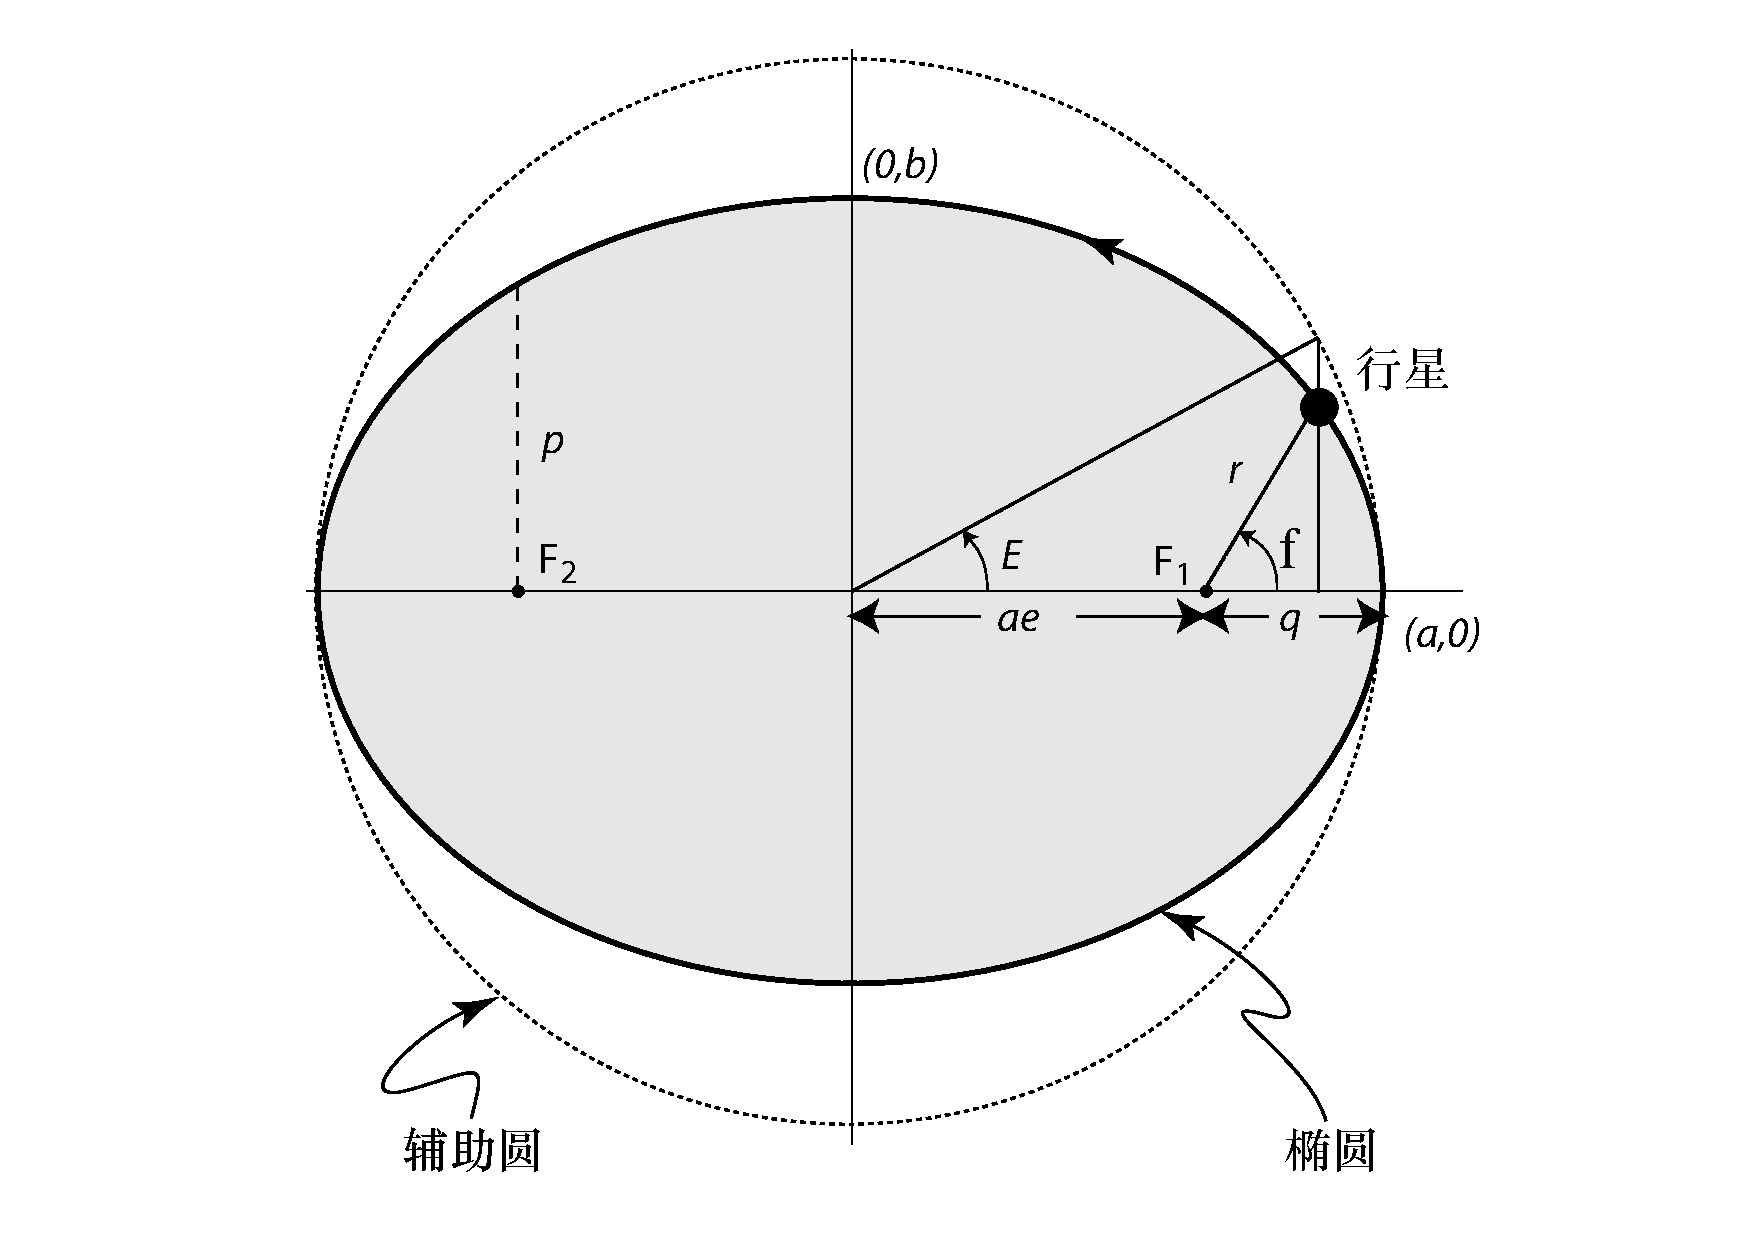
\includegraphics[width=0.95\textwidth]{figures/appendix/f1_ellipse.pdf}
\caption{二体在轨道平面内的椭圆运动示意图,图片来源 Perryman。}
\label{fig:ellipse}
\end{figure}

在次方反比的中心引力作用下,二体的运动轨迹为封闭的圆锥曲线\cite{Newton1687}。
图\ref{fig:ellipse} 和 \ref{fig:3dorbit} 展示的是椭圆二体运动示意图,其中 $a,\,e,\,i,\,\omega,\,\Omega,\,f$ 
被称作描述椭圆二体运动的六个轨道常数,文内符号几乎均沿袭自书本\citen{MurrayDermott1999ssd}。
在中心天体坐标系中,行星距离主星的标量距离 $r$ 可表示为:
\begin{equation} \label{radialdistance}
r = \frac{a(1-e^2)}{1+e\cos f}
\end{equation} %\myequation{二体运动的径向距离与轨道根素的关系}

\begin{figure}[t]
\centering
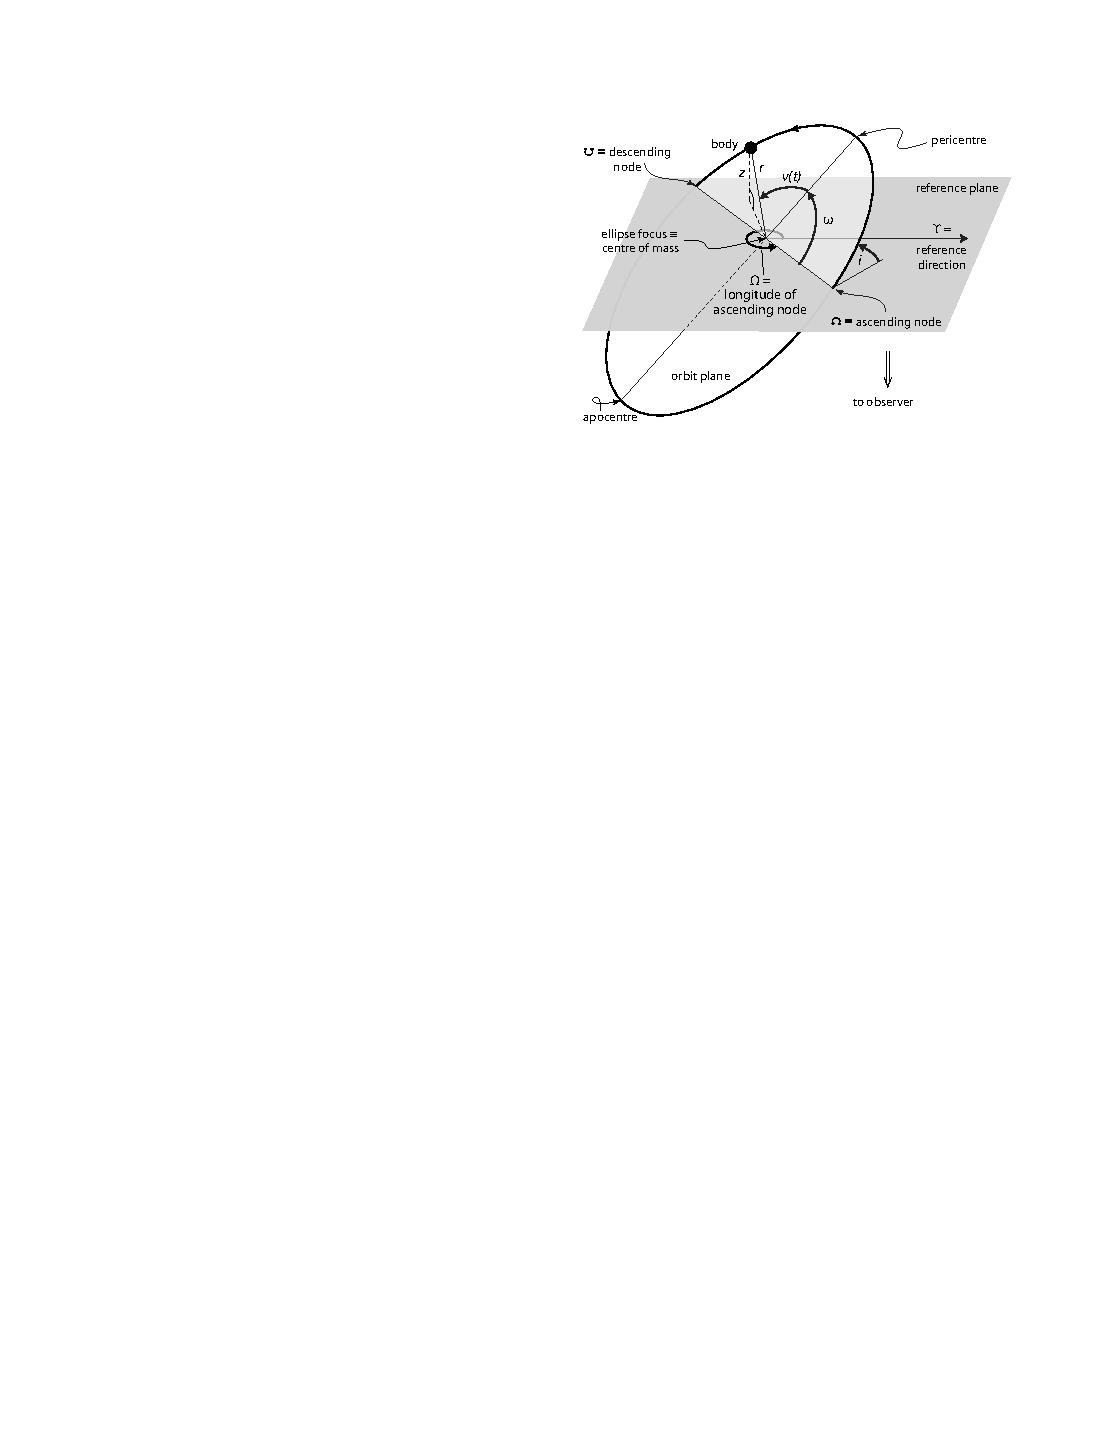
\includegraphics[width=0.85\textwidth]{figures/appendix/f2_3dorbit.pdf}
\caption{椭圆二体运动轨道在三维空间内的示意图,图内标识分别为轨道根数与参考系。图片来源 Perryman。}
\label{fig:3dorbit}
\end{figure}

\begin{figure}[hb!]
\centering
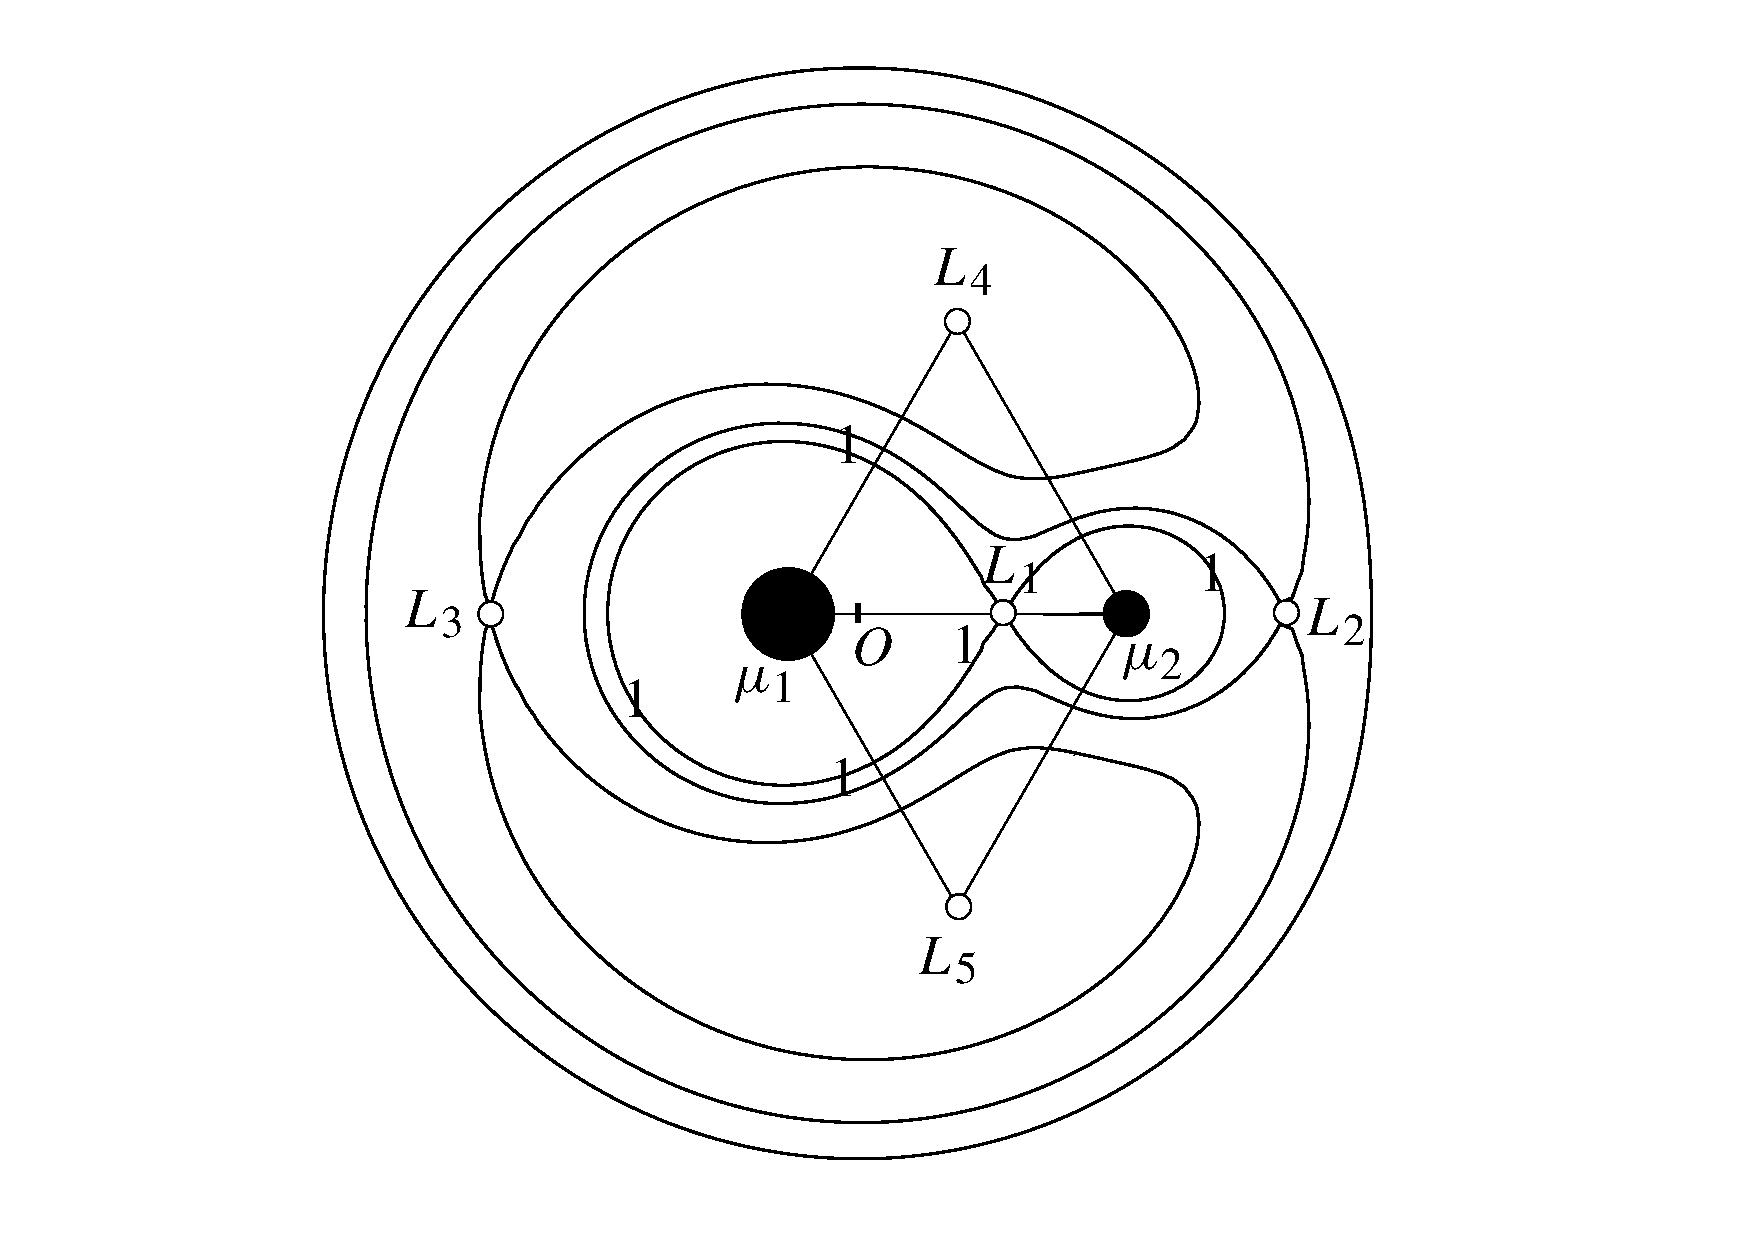
\includegraphics[width=0.75\textwidth]{figures/appendix/f3_rochelimit.pdf}
\caption[双星中洛希瓣的示意图,伴星主星质量比 $\mu_2/\mu_1 = 0.2$,其中 $L_1$ 被称为第一朗格朗日点,穿过它的等引力势面(用数字 1 来标注)分别被称作两颗星的洛希半径。图片版权 C. D. Murray,S. F. Dermott]{双星中洛希瓣的示意图,伴星主星质量比 $\mu_2/\mu_1 = 0.2$,其中 $L_1$ 被称为第一朗格朗日点,穿过它的等引力势面(用数字 1 来标注)分别被称作两颗星的洛希半径。图片来源书籍 \citen{MurrayDermott1999ssd}。}
\label{fig:rocher}
\end{figure}

\chapter{赫罗图} \label{apdx:HRdiagram}
\begin{figure}[ht!]
\centering
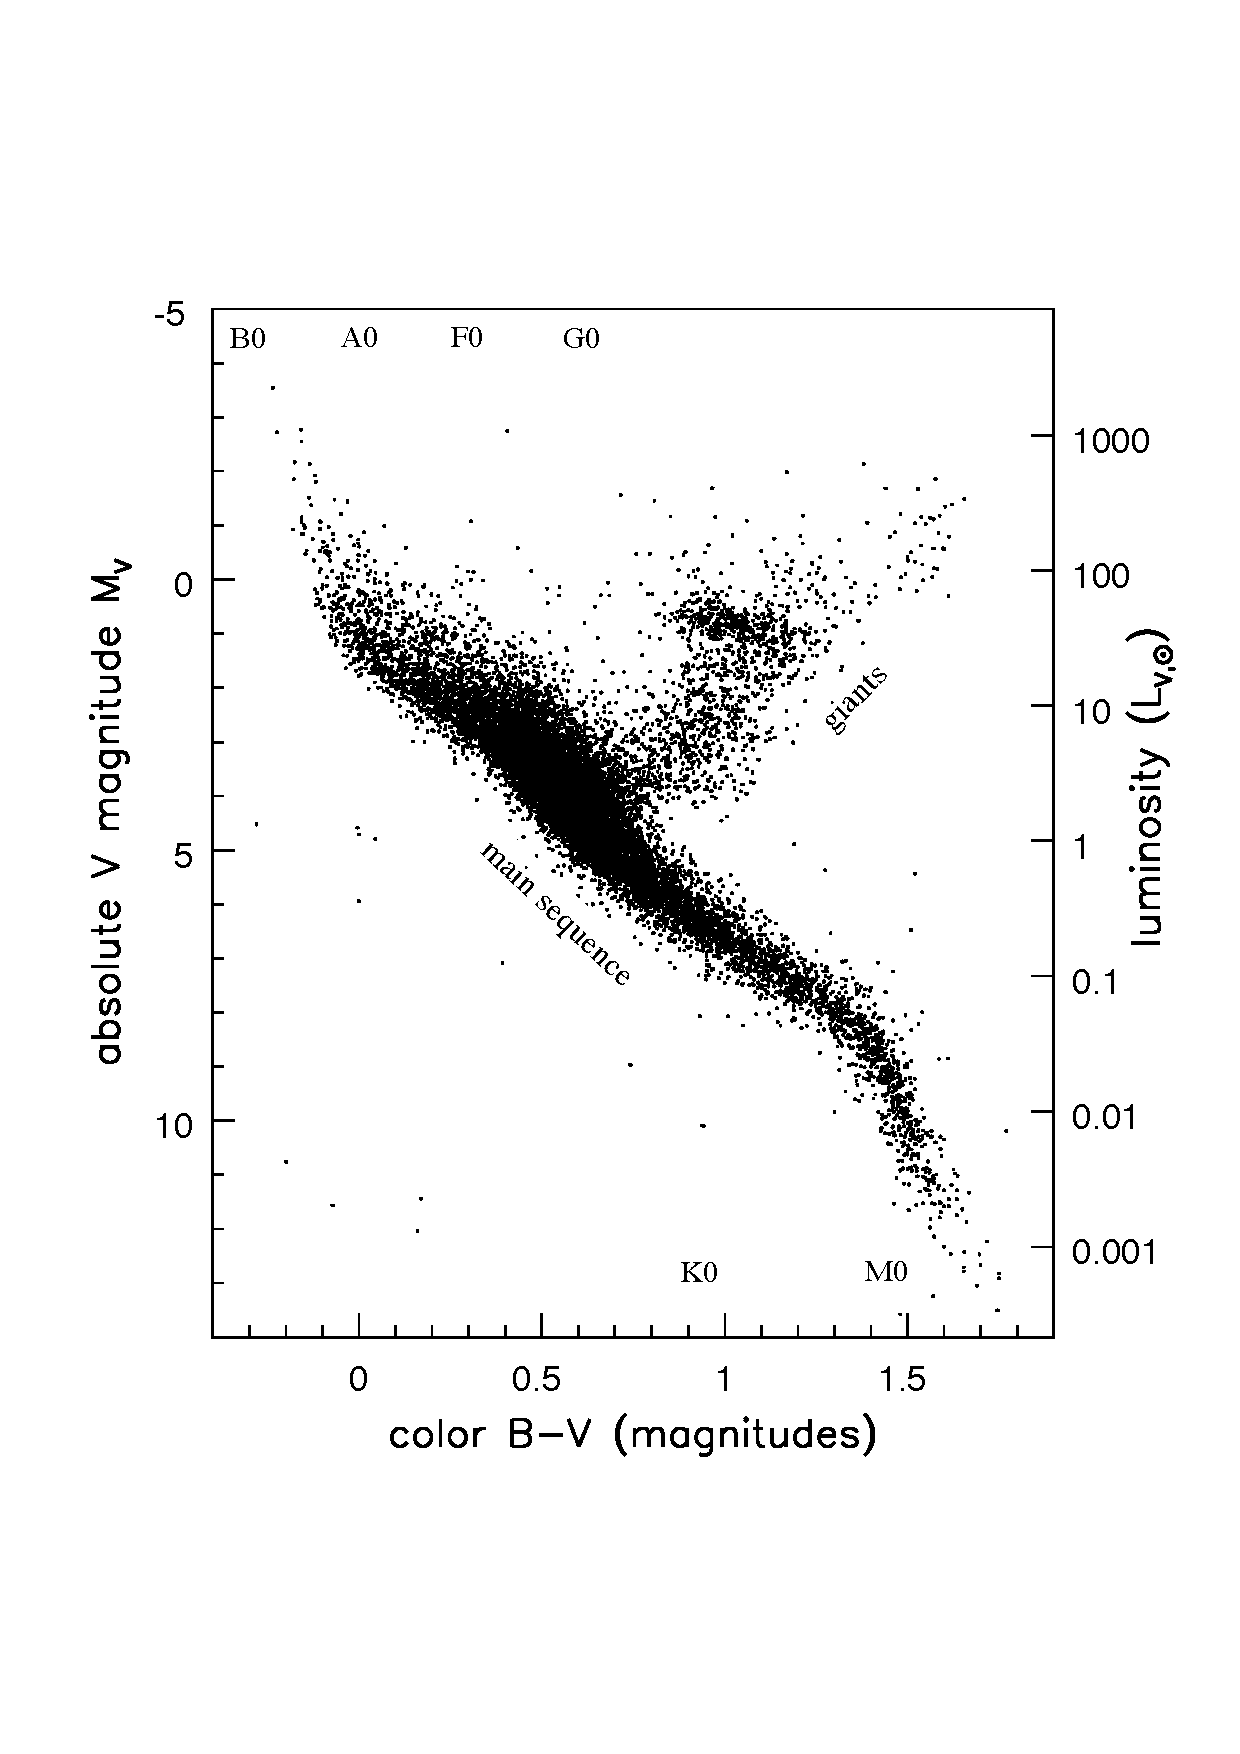
\includegraphics[width=0.97\textwidth]{figures/appendix/f4_HRdiagram.pdf}
\caption[赫罗图示意图,数据采自 ESA/Hipparcos/Tycho]{太阳附近恒星赫罗图示意图,纵坐标 V 波段绝对星等,横坐标 B-V 色指数。另外按照色指数不同分别标注了恒星光谱型(BAFGKM --- 0),以及绝对星等对应的恒星光度(右侧纵坐标),可以看到临近恒星主要分为主序以及巨星支。 数据来源文献 \citen{Hipparcos1997}。}
\label{fig:hrdiagram}
\end{figure}


